\documentclass[12pt,a4paper]{article}
\usepackage[T1]{fontenc}
\usepackage[spanish,es-nodecimaldot]{babel}
\usepackage{tgtermes}
\usepackage{newtxmath}
\usepackage{amsmath}
\usepackage{textcomp}
\usepackage{graphicx}
\usepackage{geometry}
\usepackage{xcolor}
\usepackage{setspace}
\usepackage{titlesec}
\usepackage{tocloft}
\usepackage{fancyhdr}
\usepackage{enumitem}
\usepackage{hyperref}

\geometry{margin=2.5cm}

\definecolor{AzulPrincipal}{HTML}{0B2D4D}
\definecolor{AzulSecundario}{HTML}{1F5F8B}
\definecolor{OroAcento}{HTML}{C9A227}
\definecolor{GrisTexto}{HTML}{444444}

\hypersetup{
    colorlinks=true,
    linkcolor=black,
    urlcolor=black,
    citecolor=black,
    pdftitle={Plantilla de Informe},
    pdfauthor={Tu Nombre}
}

\setlength{\parindent}{1.25cm}
\setlength{\parskip}{0.25em}
\onehalfspacing

\setlist[itemize]{leftmargin=2.8em, labelsep=0.8em, topsep=0.35em, itemsep=0.2em}
\setlist[enumerate]{leftmargin=1.7em, topsep=0.35em, itemsep=0.2em}

\titleformat{\section}[hang]{\fontsize{18pt}{22pt}\selectfont\normalfont\color{black}}{\thesection.}{0.8em}{}
\titleformat{\subsection}[hang]{\fontsize{14pt}{17pt}\selectfont\normalfont\color{black}}{\thesubsection}{0.8em}{}

\renewcommand{\cftsecfont}{\normalfont}
\renewcommand{\cftsecpagefont}{\normalfont}
\renewcommand{\cftsubsecfont}{\normalfont}
\renewcommand{\cftsubsecpagefont}{\normalfont}
\renewcommand{\cftsecleader}{\cftdotfill{\cftdotsep}}
\renewcommand{\cftsubsecleader}{\cftdotfill{\cftdotsep}}
\renewcommand{\contentsname}{Índice}
\renewcommand{\cfttoctitlefont}{\hfill\normalfont\fontsize{18pt}{22pt}\selectfont}
\renewcommand{\cftaftertoctitle}{\hfill}

\titlespacing*{\section}{0pt}{1.1em}{0.55em}
\titlespacing*{\subsection}{0pt}{0.9em}{0.35em}

\setlength{\headheight}{30pt}

\pagestyle{fancy}
\fancyhf{}
\lhead{\small\textcolor{black!65}{\Laboratorio: \Tema}}
\rhead{}
\cfoot{\small\textcolor{black}{\thepage}}
\renewcommand{\headrulewidth}{0.4pt}
\renewcommand{\headrule}{\hbox to\headwidth{\color{black!65}\leaders\hrule height \headrulewidth\hfill}}
\renewcommand{\footrulewidth}{0pt}

\providecommand{\Universidad}{UNIVERSIDAD NACIONAL DE INGENIERÍA}
\providecommand{\Facultad}{FACULTAD DE CIENCIAS}
\providecommand{\Escuela}{ESCUELA DE FÍSICA}
\providecommand{\Curso}{CIRCUITOS ELÉCTRICOS ANALÓGICOS}
\providecommand{\Seccion}{SECCIÓN A}
\providecommand{\NumeroLaboratorio}{X}
\providecommand{\Laboratorio}{LABORATORIO N\textdegree{} \NumeroLaboratorio}
\providecommand{\Tema}{TÍTULO DE LA PRÁCTICA}
\providecommand{\RutaLogo}{logo.PNG}
\providecommand{\IntegrantesBloque}{%
\begin{enumerate}[leftmargin=1.8em,label=\arabic*.]
    \item Integrante 1 -- código
    \item Integrante 2 -- código
\end{enumerate}}
\providecommand{\FechaRealizacion}{Fecha de realización: dd de mes de aaaa - hh:mm}
\providecommand{\Ciudad}{LIMA - PERU}

\newcommand{\ConfigurarInforme}[3]{%
    \renewcommand{\NumeroLaboratorio}{#1}%
    \renewcommand{\Tema}{#2}%
    \renewcommand{\FechaRealizacion}{#3}%
}

\newcommand{\ConfigurarIntegrantes}[1]{%
    \renewcommand{\IntegrantesBloque}{#1}%
}

\providecommand{\tituloSeccion}[1]{\section{#1}}

\providecommand{\makeInformePortada}{%
\begin{titlepage}
    \thispagestyle{empty}
    \vspace*{0.65cm}
    \begin{center}
        {\Large\bfseries\color{OroAcento} \Universidad}\par
        \vspace{0.45cm}
        {\Large\bfseries\color{AzulPrincipal} \Facultad}\par
        \vspace{0.25cm}
        {\Large\bfseries\color{AzulPrincipal} \Escuela}\par
    \end{center}

    \vspace{0.1cm}
    \begin{center}
        \includegraphics[width=0.4\textwidth]{\RutaLogo}%
    \end{center}

    \vspace{0.01cm}
    \begin{center}
        {\Large\bfseries\color{AzulPrincipal} \Curso}\par
        \vspace{0.35cm}
        {\Large\bfseries\color{red} \Seccion}\par
    \end{center}

    \vspace{0.1cm}
    \begin{center}
        {\large\bfseries \Laboratorio: \Tema}\par
    \end{center}

    \vspace{0.55cm}
    \noindent{\large\textbf{INTEGRANTES DE LA MESA:} 2}\par
    \vspace{0.35cm}
    \begingroup
    \leftskip=1.15cm
    \rightskip=1.15cm
    \parindent=0pt
    \IntegrantesBloque
    \endgroup

    \vspace{0.55cm}
    \begin{center}
        {\FechaRealizacion}\par
    \end{center}

    \vfill

    \begin{center}
        {\large\bfseries \Ciudad}
    \end{center}
\end{titlepage}
}
\usepackage{tikz}
\usepackage{pgfplots}
\pgfplotsset{compat=1.18}
\renewcommand{\RutaLogo}{../../PLANTILLA/logo.PNG}
\graphicspath{{Imagenes/}}
\ConfigurarInforme{7}{CIRCUITOS BÁSICOS CON DIODOS}{Fecha de realización del Laboratorio N\textdegree{}7: 28 de Abril del 2026}

% Inicio del informe
\begin{document}
\makeInformePortada
\setcounter{page}{1}
\tableofcontents
\newpage

% --- Contenido añadido: Objetivos y Fundamento teorico ---
\section{Objetivos}
\subsection{Objetivo General}
Estudiar el comportamiento de diodos semiconductores.

\subsection{Objetivos Específicos}
\begin{enumerate}
\item Analizar el comportamiento de un diodo semiconductor en un circuito alimentado por una fuente AC.
\item Estudiar los circuitos rectificadores de media onda y onda completa.
\end{enumerate}

\section{Fundamento teórico}
Un semiconductor es un material cuya conductividad eléctrica es intermedia entre la de un conductor y la de un aislante. En estado puro tiene pocos portadores libres, y su conductividad puede modificarse mediante dopaje. En este laboratorio interesa el comportamiento no lineal del diodo y su uso en rectificación.

\subsection{Diodo}
El diodo conduce en polarización directa y bloquea en polarización inversa, con una pequeña corriente de saturación inversa. Su comportamiento corriente--voltaje se describe con la ecuación de Shockley:
\begin{equation}
I = I_s\left(e^{\frac{V}{\eta V_T}} - 1\right)
\end{equation}
donde $I_s$ es la corriente de saturación, $\eta$ es el factor de idealidad y $V_T$ es la tensión térmica, que a 300 K vale aproximadamente 26 mV.

Para el análisis práctico se usan tres aproximaciones: diodo ideal, aproximación de umbral y aproximación con resistencia interna.

\subsection{Rectificadores y rizado}

Los rectificadores convierten una señal alterna en una señal continua pulsante. En el rectificador de media onda ideal, para una señal senoidal de amplitud $V_0$:
\begin{equation}
\overline{V}_{out}=\frac{V_0}{\pi}
\end{equation}
\begin{equation}
V_{out,ef}=\frac{V_0}{2}
\end{equation}
\begin{equation}
r=\sqrt{\left(\frac{\pi}{2}\right)^2-1}\approx1.21
\end{equation}

En el rectificador de onda completa ideal con puente de diodos:
\begin{equation}
\overline{V}_{out}=\frac{2V_0}{\pi}
\end{equation}
\begin{equation}
V_{out,ef}=\frac{V_0}{\sqrt{2}}
\end{equation}
\begin{equation}
r\approx0.48
\end{equation}

Si se agrega un capacitor en paralelo con la carga, el condensador se carga cerca del valor pico y se descarga entre máximos consecutivos. En ese caso, el voltaje de rizado se define como la variación periódica de la salida respecto al valor promedio:
\begin{equation}
v_r(t)=v_{out}(t)-\overline{V}_{out}
\end{equation}

En lo que sigue, $V_r$ denota el valor pico a pico del rizado:
\begin{equation}
V_r\equiv V_{r(pp)}
\end{equation}

Para deducir el rizado en un rectificador con filtro capacitivo, se analiza la descarga del capacitor entre picos consecutivos. Cuando el voltaje rectificado alcanza un máximo, el capacitor se carga aproximadamente hasta el valor pico $V_p$. Luego, entre dos máximos consecutivos, los diodos dejan de conducir y el capacitor se descarga a través de la resistencia de carga.

La corriente del capacitor está dada por:
\begin{equation}
i_C=C\frac{dv}{dt}
\end{equation}

Bajo la aproximación de rizado pequeño, la corriente en la carga puede considerarse aproximadamente constante durante la descarga, de modo que:
\begin{equation}
i_C\approx -I_L
\end{equation}

Por lo tanto:
\begin{equation}
-I_L=C\frac{dv}{dt}
\end{equation}

y despejando:
\begin{equation}
\frac{dv}{dt}=-\frac{I_L}{C}
\end{equation}

Integrando entre dos instantes consecutivos de recarga del capacitor:
\begin{equation}
\Delta V\approx\frac{I_L\Delta t}{C}
\end{equation}

Como el tiempo entre recargas es:
\begin{equation}
\Delta t=T_r=\frac{1}{f_r}
\end{equation}

se obtiene:
\begin{equation}
V_r\approx\frac{I_L}{f_rC}
\end{equation}

Para un rectificador de media onda:
\begin{equation}
f_r=f
\end{equation}

mientras que para un rectificador de onda completa:
\begin{equation}
f_r=2f
\end{equation}

Por tanto, para onda completa:
\begin{equation}
V_r\approx\frac{I_L}{2fC}
\end{equation}

Además, usando:
\begin{equation}
I_L\approx\frac{V_{DC}}{R_L}
\end{equation}

también puede escribirse:
\begin{equation}
V_r\approx\frac{V_{DC}}{R_Lf_rC}
\end{equation}

y para onda completa:
\begin{equation}
V_r\approx\frac{V_{DC}}{2fR_LC}
\end{equation}

Si la descarga del capacitor se aproxima mediante una onda triangular, el valor eficaz del rizado viene dado por:
\begin{equation}
V_{r,ef}=\frac{V_{r(pp)}}{2\sqrt{3}}
\end{equation}

En consecuencia, al aumentar la capacitancia $C$ o la resistencia de carga $R_L$, disminuye el voltaje de rizado.

\tituloSeccion{Materiales e indicaciones}
\begin{itemize}
	\item Multímetro: Instrumento de medición utilizado para verificar los valores de resistencia de los componentes, así como para medir voltajes en el circuito. 
	\item Osciloscopio: Instrumento de medición que permite visualizar en tiempo real la forma de onda de las señales de entrada y salida del circuito. 
    \item Resistencias: Son componentes que limitan el flujo de corriente en un circuito. Para su uso, se deben identificar sus valores utilizando el código de colores o un multímetro, y conectarlas en el circuito según sea necesario.
    \item Capacitores: Son componentes que almacenan energía eléctrica en forma de campo eléctrico. Para su uso, se deben identificar sus valores utilizando el código de colores o un multímetro, y conectarlos en el circuito según sea necesario.
    \item Protoboard: Es una placa de pruebas que permite realizar conexiones temporales sin necesidad de soldar. Para su uso, se deben insertar los componentes en las filas y columnas correspondientes, y realizar las conexiones utilizando cables de puente.
\end{itemize}

\section{Procedimiento experimental}
\subsection{Paso 1}
\begin{enumerate}
    \item Se construyó el circuito rectificador de media onda mostrado en la figura \ref{fig:rectificador_medio_onda} utilizando un diodo, una resistencia de carga, un generador de señales AC e identificando el punto de referencia (GND) de manera adecuada.
    \begin{figure}[H]
        \centering
        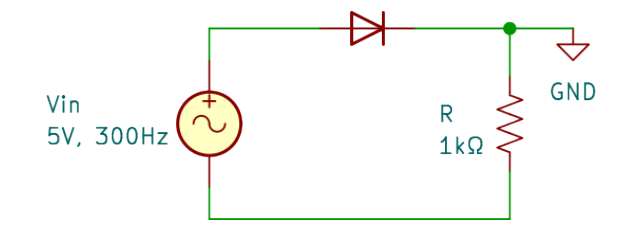
\includegraphics[width=0.5\linewidth]{imagen1.png}
        \caption{Circuito rectificador de media onda. [2]}
        \label{fig:rectificador_medio_onda}
    \end{figure}
    \item Se conectó el CH1 del osciloscopio en el voltaje del diodo $V_D$ y el voltaje de la resistencia $V_R$ en el CH2.
    \item Se configuró el osciloscopio en modo XY para observar la curva característica del diodo (invirtiendo CH2).
    \item Se tomó una captura de pantalla del osciloscopio.
\end{enumerate}

\subsection{Paso 2}
\begin{enumerate}
    \item Se construyó el circuito rectificador de media onda de la figura \ref{fig:rectificador_medio_onda2} utilizando un diodo, una resistencia de carga, un generador de señales AC e identificando el punto de referencia (GND) de manera adecuada.
    \begin{figure}[H]
        \centering
        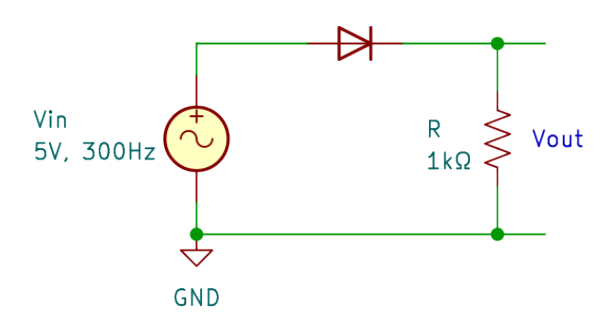
\includegraphics[width=0.5\linewidth]{imagen2.png}
        \caption{Segundo circuito rectificador de media onda. [2]}
        \label{fig:rectificador_medio_onda2}
    \end{figure}
    \item Se conectó el CH1 del osciloscopio en el voltaje de entrada $V_{in}$ y el voltaje de salida $V_{out}$ (a través de la resistencia) al CH2. Se midió los voltajes pico de cada señal.
    \item Se tomó una captura de pantalla del osciloscopio.
\end{enumerate}
\newpage
\subsection{Paso 3}
\begin{enumerate}
    \item Se construyó el circuito de la figura \ref{fig:rectificador_medio_onda3} utilizando un diodo, una resistencia de carga, un generador de señales AC, una fuente de voltaje y se identificó el punto de referencia (GND) de manera adecuada.
    \begin{figure}[H]
        \centering
        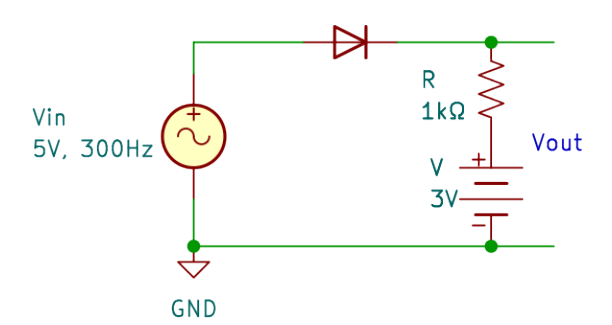
\includegraphics[width=0.5\linewidth]{imagen3.png}
        \caption{Circuito rectificador de media onda con fuente de voltaje. [2]}
        \label{fig:rectificador_medio_onda3}
    \end{figure}
    \item Se configuró el osciloscopio en modo DC, se conectó el CH1 del osciloscopio en el voltaje de entrada $V_{in}$ y el voltaje de salida $V_{out}$ al CH2. 
    \item Se tomó una captura de la señal de salida en el osciloscopio.
    \item Se invirtió el diodo (figura \ref{fig:rectificador_medio_onda4}) y se repitieron los pasos anteriores.
    \begin{figure}[H]
        \centering
        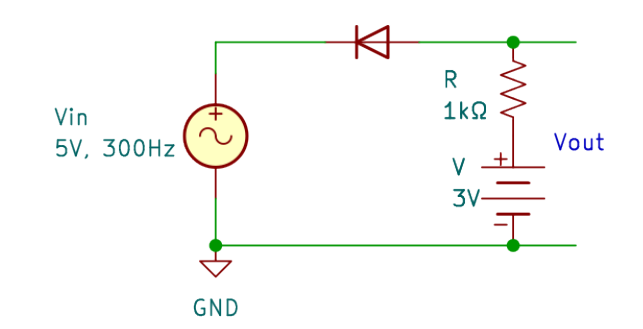
\includegraphics[width=0.5\linewidth]{imagen4.png}
        \caption{Circuito rectificador de media onda con diodo invertido. [2]}
        \label{fig:rectificador_medio_onda4}
    \end{figure}
\end{enumerate}

\subsection{Paso 4}
\begin{enumerate}
    \item Se construyó el circuito rectificador de onda completa de la figura \ref{fig:rectificador_onda_completa} utilizando cuatro diodos, una resistencia de carga, un generador de señales AC e identificando el punto de referencia (GND) de manera adecuada.
    \begin{figure}[H]
        \centering
        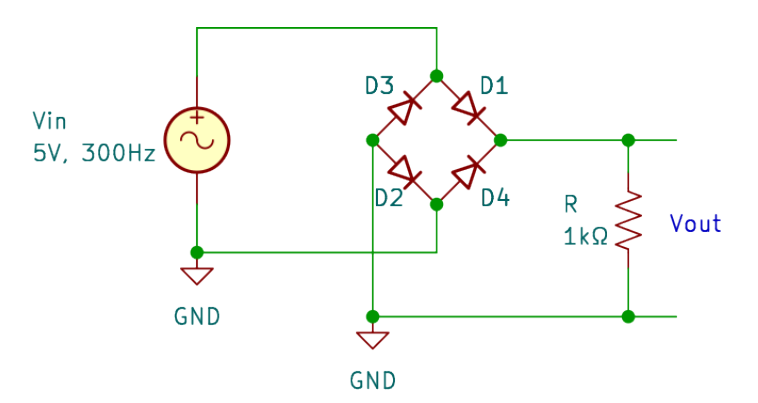
\includegraphics[width=0.5\linewidth]{imagen5.png}
        \caption{Circuito rectificador de onda completa. [2]}
        \label{fig:rectificador_onda_completa}
    \end{figure}
    \item Se conectó el CH1 del osciloscopio en el voltaje de entrada $V_{in}$ y el voltaje de salida $V_{out}$ al CH2.
    \item Se trató de verificar si es posible observar ambas señales de manera simultánea en el osciloscopio.
    \item Se tomaron capturas de pantalla del osciloscopio.
\end{enumerate}

\subsection{Paso 5}
\begin{enumerate}
    \item Se agregó al circuito anterior un filtro pasa-baja, como se muestra en la figura \ref{fig:rectificador_onda_completa_filtro}, utilizando un capacitor en paralelo con la resistencia de carga.
    \begin{figure}[H]
        \centering
        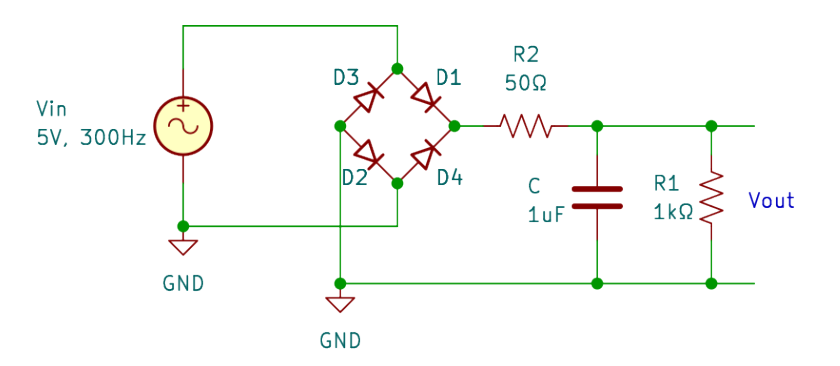
\includegraphics[width=0.6\linewidth]{imagen6.png}
        \caption{Circuito rectificador de onda completa con filtro capacitivo. [2]}
        \label{fig:rectificador_onda_completa_filtro}
    \end{figure}
    \item Se conectó el CH1 del osciloscopio en el voltaje de entrada $V_{in}$ y el voltaje de salida $V_{out}$ al CH2.
    \item Se observó la señal de salida en el osciloscopio: se midió la componente DC y AC de la señal.
    \item Se calculó el voltaje de rizado y se tomaron capturas de pantalla del osciloscopio.
    \item Se repitió el procedimiento anterior para tres valores distintos de capacitancia: $1\ \mu\mathrm{F}$, $10\ \mu\mathrm{F}$ y $47\ \mu\mathrm{F}$.
\end{enumerate}

\tituloSeccion{Análisis de datos}
\subsection{Paso 1}
Curva característica del diodo:
\begin{figure}[H]
    \centering
    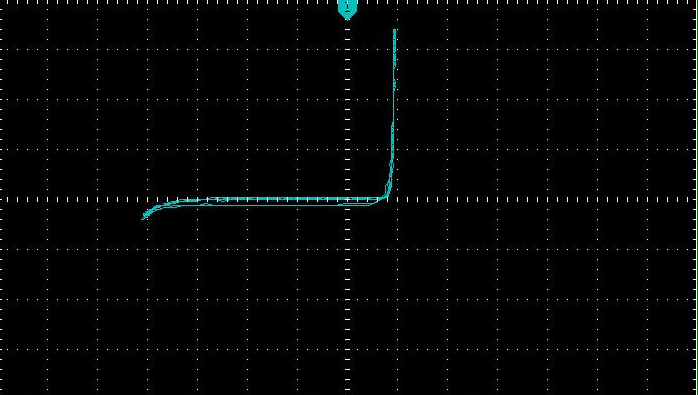
\includegraphics[width=0.6\linewidth]{imagen7.png}
    \caption{Curva característica del diodo obtenida en el osciloscopio.}
    \label{fig:curva_diodo}
\end{figure}

El diodo empieza a conducir a partir de un voltaje umbral de aproximadamente $0,7\,$V, lo cual es consistente con el comportamiento esperado para un diodo de silicio. En la región de polarización directa, la corriente aumenta exponencialmente con el voltaje aplicado, mientras que en la región de polarización inversa, la corriente se mantiene muy baja (corriente de saturación inversa) hasta alcanzar una tensión de ruptura.

\subsection{Paso 2}
Señal de salida del rectificador de media onda y su amplitud pico:
\begin{figure}[H]
    \centering
    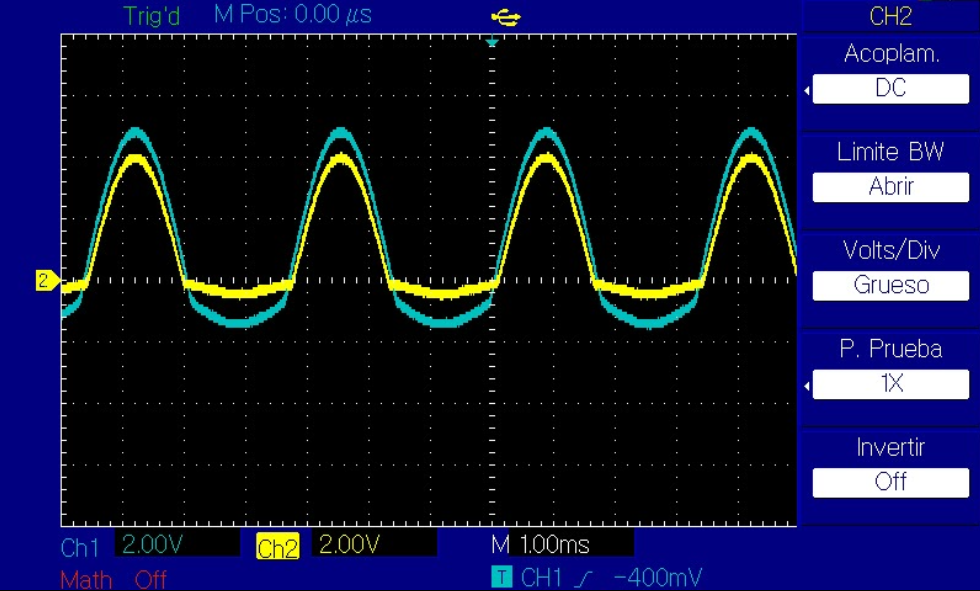
\includegraphics[width=0.7\linewidth]{imagen8.png}
    \caption{Señal de entrada y salida del rectificador de media onda.}
    \label{fig:salida_medio_onda}
\end{figure}
Los voltajes pico respectivos de la señal de entrada y salida son aproximadamente $5\,$V y $4,3\,$V, lo cual es consistente con la caída de tensión en el diodo (aproximadamente $0,7\,$V) y la forma de onda rectificada que se espera para un circuito de media onda.: 

\subsection{Paso 3}
Señal de salida del rectificador de media onda con fuente de voltaje y diodo:
\begin{figure}[H]
    \centering
    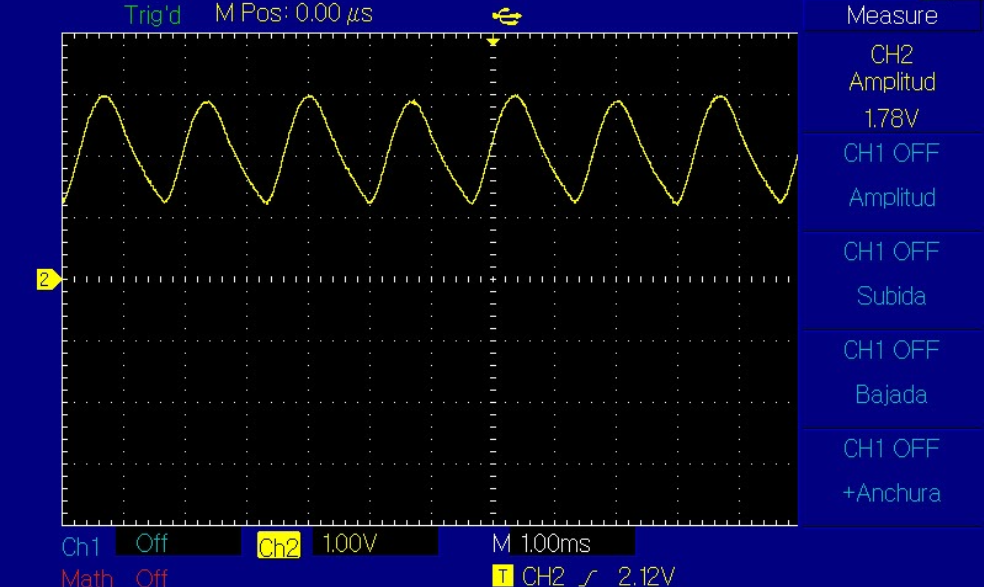
\includegraphics[width=0.7\linewidth]{imagen10.png}
    \caption{Señal de salida del rectificador de media onda con fuente de voltaje y diodo.}
    \label{fig:salida_medio_onda_fuente}
\end{figure}
Señal de salida del rectificador de media onda con fuente de voltaje y diodo invertido:
\begin{figure}[H]
    \centering
    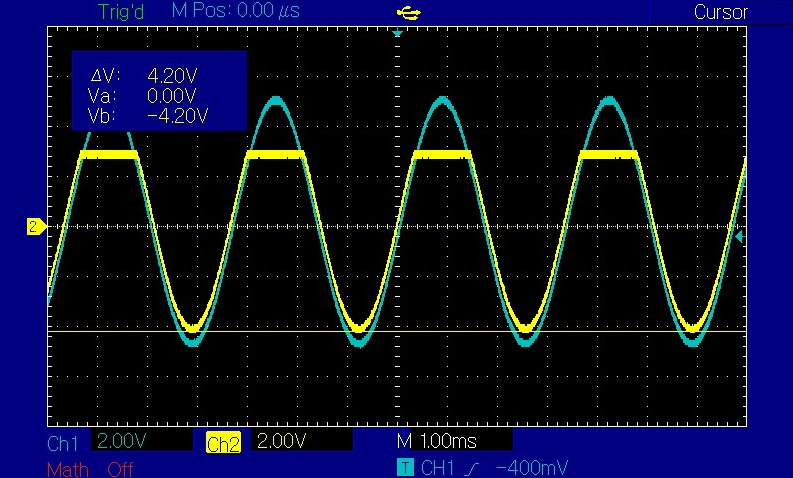
\includegraphics[width=0.7\linewidth]{imagen11.png}
    \caption{Señal de salida del rectificador de media onda con fuente de voltaje y diodo invertido.}
    \label{fig:salida_medio_onda_fuente_invertido}
\end{figure}
En la figura \ref{fig:salida_medio_onda_fuente} se observa el funcionamiento de un recortador (clipper) de serie polarizado, donde la señal de salida elimina los voltajes inferiores al nivel de la fuente (en este caso, \(3\,\)V), permitiendo solo el paso de los picos superiores. Por otro lado, en la figura \ref{fig:salida_medio_onda_fuente_invertido}, al invertir el diodo, el circuito actúa como un recortador de picos superiores; la señal se limita al voltaje de la fuente (\(3\,\)V) cuando la entrada supera dicho umbral y mantiene la forma senoidal en el resto del ciclo. Es importante notar que ninguna de las configuraciones es un sujetador (clamp), ya que el circuito carece de un elemento reactivo (capacitor) para desplazar el nivel de DCVerificación si se pueden observar ambas señales de entrada y salida simultáneamente en el osciloscopio:

\subsection{Paso 4}
Verificación de la visualización simultánea de señales de entrada y salida en el osciloscopio: Las señales de entrada y salida no se pudieron observar simultáneamente en el osciloscopio, lo cual se atribuye a la configuración del osciloscopio y a la naturaleza de las señales. La señal de entrada es una onda senoidal alterna, mientras que la señal de salida es una onda rectificada que solo contiene los semiperiodos positivos. Esto puede dificultar la visualización simultánea debido a las diferencias en amplitud y forma de onda.

Señal de entrada del rectificador de onda completa:
\begin{figure}[H]
    \centering
    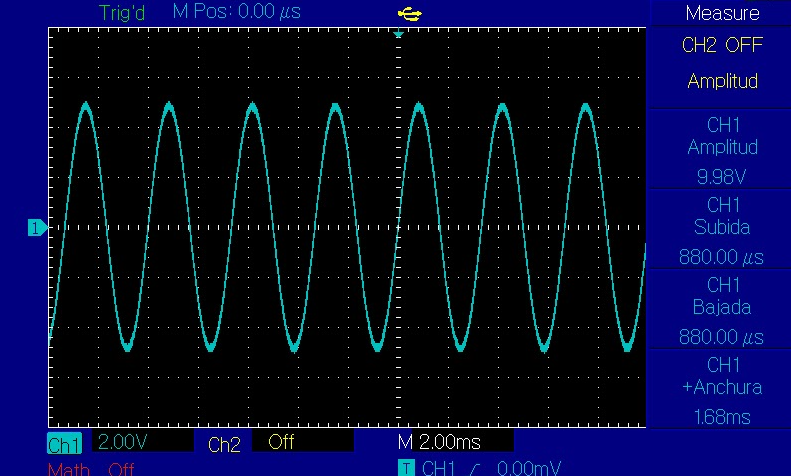
\includegraphics[width=0.7\linewidth]{imagen12.png}
    \caption{Señal de entrada del rectificador de onda completa.}
    \label{fig:entrada_onda_completa}
\end{figure}

Señal de salida del rectificador de onda completa:
\begin{figure}[H]
    \centering
    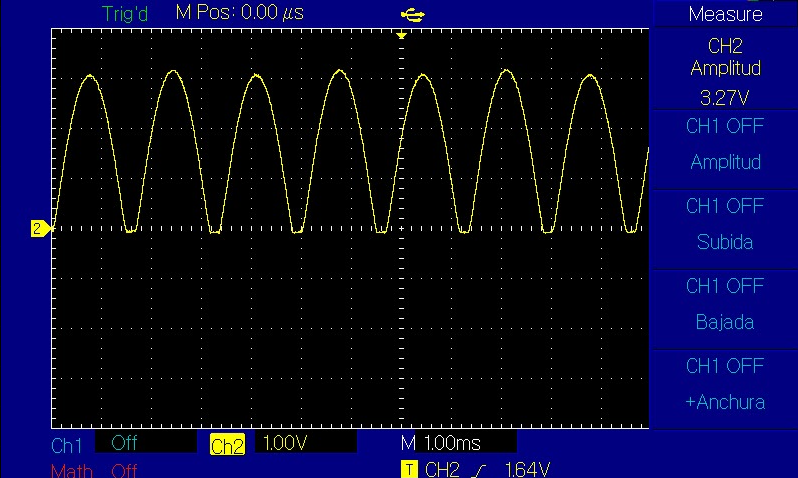
\includegraphics[width=0.7\linewidth]{imagen13.png}
    \caption{Señal de salida del rectificador de onda completa.}
    \label{fig:salida_onda_completa}
\end{figure}

\newpage
\subsection{Paso 5}
Señal de salida del rectificador de onda completa con filtro capacitivo:
\begin{figure}[H]
    \centering
    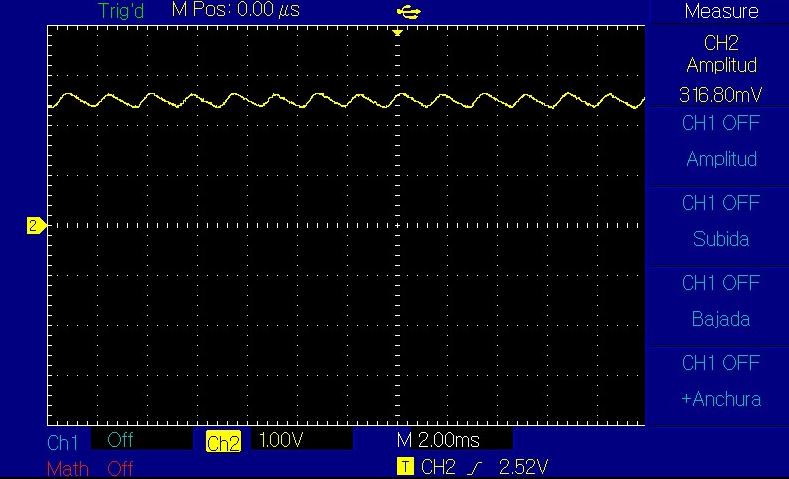
\includegraphics[width=0.7\linewidth]{imagen14.png}
    \caption{Señal de salida del rectificador de onda completa con filtro capacitivo.}
    \label{fig:salida_onda_completa_filtro}
\end{figure}

Para el rectificador de onda completa con filtro capacitivo se utiliza la expresión:
\begin{equation}
V_r\approx\frac{V_{DC}}{2fR_LC}
\end{equation}

En el circuito mostrado se tienen los siguientes datos:
\begin{equation}
V_{in}=5\,V
\end{equation}
\begin{equation}
f=300\,Hz
\end{equation}
\begin{equation}
R_2=54.9\,\Omega
\end{equation}
\begin{equation}
R_L=R_1=1\,k\Omega
\end{equation}

Como se trata de un rectificador de onda completa:
\begin{equation}
f_r=2f=600\,Hz
\end{equation}

Considerando diodos de silicio con caída aproximada de $0.7\,V$ cada uno, en el puente rectificador conducen dos diodos simultáneamente, por lo que:
\begin{equation}
V_{DC}\approx V_p-2V_D
\end{equation}

Entonces:
\begin{equation}
V_{DC}\approx 5-1.4=3.6\,V
\end{equation}

\subsubsection*{Caso 1: $C=1\,\mu F$}

\begin{equation}
V_r\approx\frac{3.6}{(600)(1000)(1\times10^{-6})}
\end{equation}
\begin{equation}
V_r\approx 6.0\,V
\end{equation}

Este resultado indica un rizado muy grande, por lo que la aproximación de rizado pequeño deja de ser válida.

\subsubsection*{Caso 2: $C=10\,\mu F$}

\begin{equation}
V_r\approx\frac{3.6}{(600)(1000)(10\times10^{-6})}
\end{equation}
\begin{equation}
V_r\approx0.60\,V
\end{equation}

\subsubsection*{Caso 3: $C=47\,\mu F$}

\begin{equation}
V_r\approx\frac{3.6}{(600)(1000)(47\times10^{-6})}
\end{equation}
\begin{equation}
V_r\approx0.128\,V
\end{equation}

Por lo tanto, los valores aproximados del voltaje de rizado son:
\begin{equation}
V_r(1\,\mu F)\approx6.0\,V
\end{equation}
\begin{equation}
V_r(10\,\mu F)\approx0.60\,V
\end{equation}
\begin{equation}
V_r(47\,\mu F)\approx0.128\,V
\end{equation}

Se observa que al aumentar la capacitancia disminuye significativamente el voltaje de rizado.

\newpage
\tituloSeccion{Actividades adicionales}
\begin{enumerate}
    \item Explique teóricamente cuál será la salida del circuito mostrado en la figura \ref{fig:rectificador_adicional} y verifique su resultado teórico mediante una simulación.
    \begin{figure}[H]
        \centering
        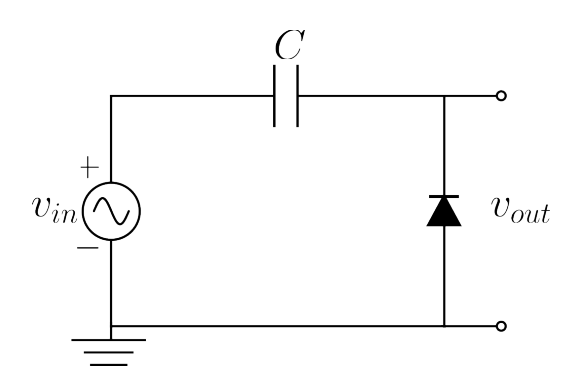
\includegraphics[width=0.4\linewidth]{imagen9.png}
        \caption{Circuito adicional para análisis teórico y simulación.}
        \label{fig:rectificador_adicional}
    \end{figure}

    Teóricamente, el circuito mostrado corresponde a un sujetador positivo con capacitor y diodo a tierra. Durante el semiciclo negativo, el diodo conduce y fija la salida cerca de 0 V, mientras el capacitor se carga hasta un valor próximo al pico de la señal de entrada. En el semiciclo positivo, el diodo queda en inversa y el capacitor conserva su carga, de modo que la señal de salida queda desplazada hacia arriba.

    Por lo tanto, la salida esperada es una onda senoidal con componente DC positiva. En el caso ideal, el valor mínimo de la salida se aproxima a 0 V y el valor máximo a aproximadamente $2V_p$; considerando la caída directa del diodo, esos valores se desplazan ligeramente. En consecuencia, el circuito no rectifica la señal, sino que la sujeta a un nivel de referencia y eleva todo el tren de onda.

    Usando un simulación en Multisim:
        \begin{figure}[H]
            \centering
            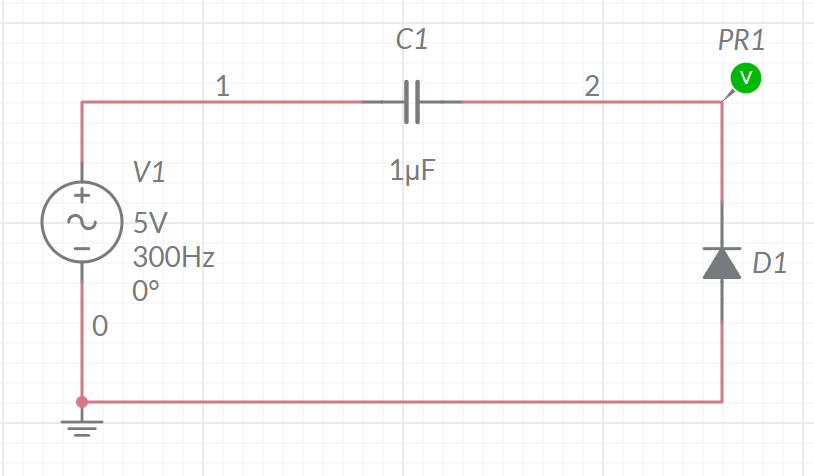
\includegraphics[width=0.7\linewidth]{imagen15.png}
            \caption{Simulación del circuito adicional en Multisim.}
            \label{fig:simulacion_rectificador_adicional}
        \end{figure}
        \newpage
        Cuya salida fue la siguiente:
        \begin{figure}[H]
            \centering
            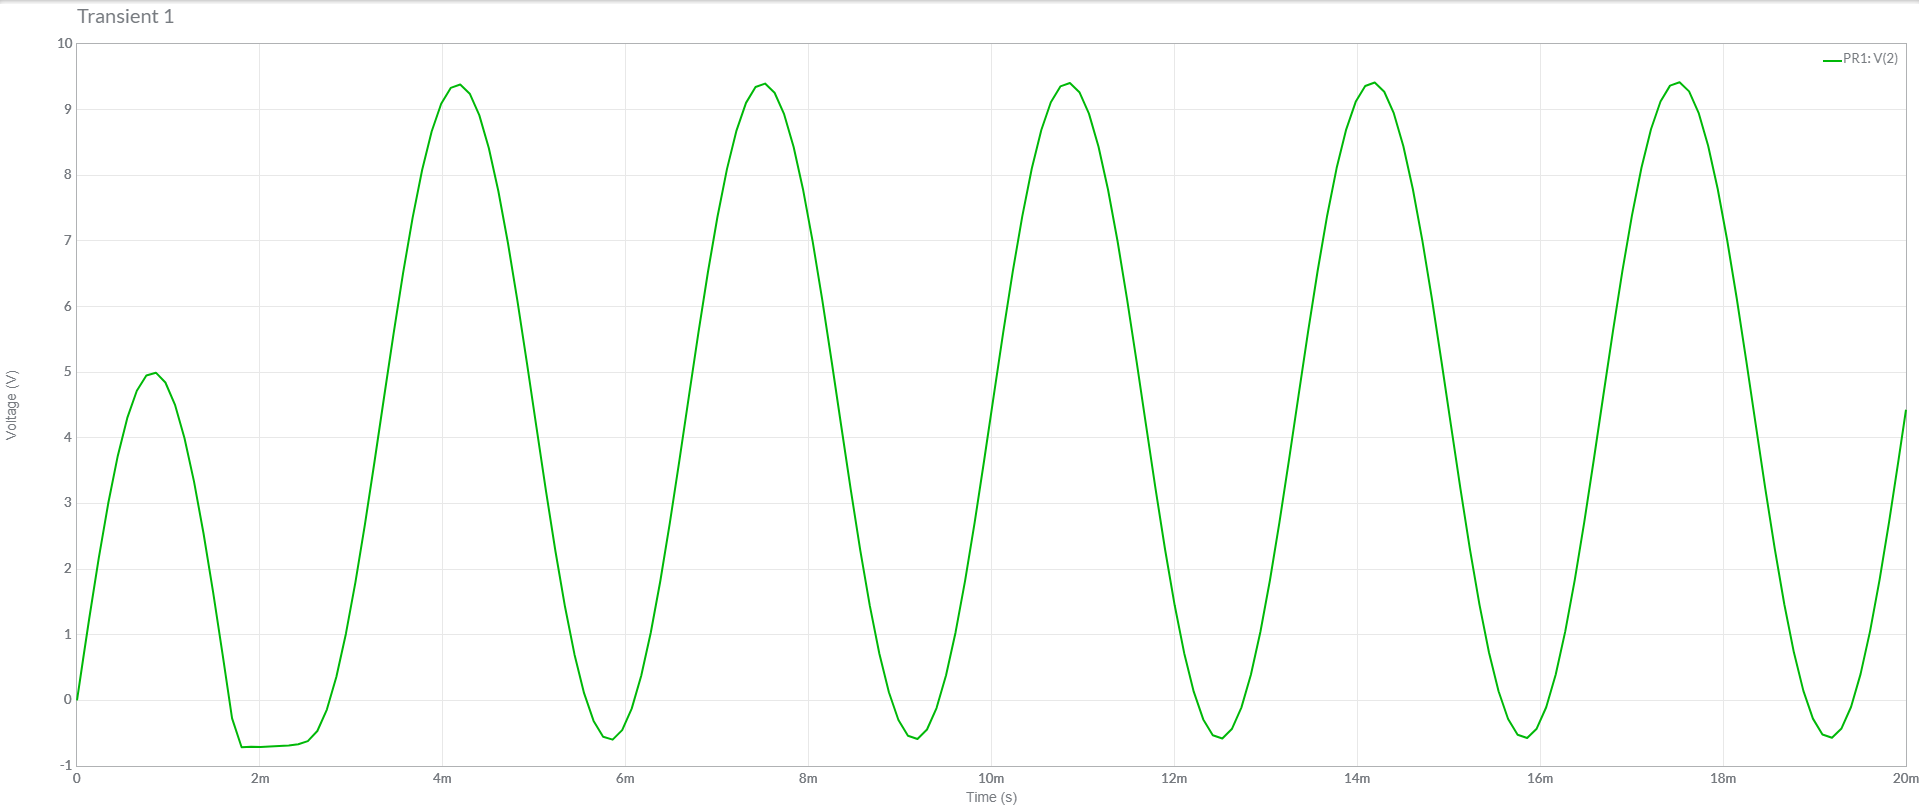
\includegraphics[width=0.7\linewidth]{imagen16.png}
            \caption{Salida del circuito adicional en la simulación.}
            \label{fig:salida_rectificador_adicional}
        \end{figure}

        La simulación en Multisim confirma el análisis teórico: la señal de salida aparece desplazada hacia arriba respecto a la entrada, con el semiciclo negativo sujeto cerca de 0 V y el semiciclo positivo elevado por la carga almacenada en el capacitor. La forma de onda obtenida coincide con el comportamiento esperado para un sujetador positivo.


        \bigskip
    \item Simular el circuito de la figura \ref{fig:rectificador_onda_completa_filtro} para diferentes valores de $R_2$ y observe como varía el voltaje de rizado. Obtenga el factor de rizado.

        Sean los siguientes valores de $R_2$:
        \begin{itemize}
            \item $R_2=75\,\Omega$
            \item $R_2=100\,\Omega$
            \item $R_2=1k\,\Omega$
            \item $R_2=10k\,\Omega$
        \end{itemize}
        
        Se hizo el experimento en el salón de laboratorio, midiendose en el osciloscopio voltajes de rizado correspondientes a:
        \begin{itemize}
            \item $R_2=75\,\Omega$: $V_r\approx1,8\,V$
            \item $R_2=100\,\Omega$: $V_r\approx1,9\,V$
            \item $R_2=1k\,\Omega$: $V_r\approx0,7\,V$
            \item $R_2=10k\,\Omega$: $V_r\approx0,1\,V$
        \end{itemize}
        \subsubsection*{Caso 1: $R_2=10\,\Omega$}

Con:
\begin{equation}
V_{r(pp)}=1.9\,V
\end{equation}

se obtiene:
\begin{equation}
V_{r,ef}=\frac{1.9}{2\sqrt{3}}\approx0.548\,V
\end{equation}

Por tanto:
\begin{equation}
r=\frac{0.548}{3.6}\approx0.152
\end{equation}
\newpage
\subsubsection*{Caso 2: $R_2=75\,\Omega$}

Con:
\begin{equation}
V_{r(pp)}=1.8\,V
\end{equation}

se obtiene:
\begin{equation}
V_{r,ef}=\frac{1.8}{2\sqrt{3}}\approx0.520\,V
\end{equation}

Por tanto:
\begin{equation}
r=\frac{0.520}{3.6}\approx0.144
\end{equation}

\subsubsection*{Caso 3: $R_2=1\,k\Omega$}

Con:
\begin{equation}
V_{r(pp)}=0.7\,V
\end{equation}

se obtiene:
\begin{equation}
V_{r,ef}=\frac{0.7}{2\sqrt{3}}\approx0.202\,V
\end{equation}

Por tanto:
\begin{equation}
r=\frac{0.202}{3.6}\approx0.056
\end{equation}

\subsubsection*{Caso 4: $R_2=10\,k\Omega$}

Con:
\begin{equation}
V_{r(pp)}=0.1\,V
\end{equation}

se obtiene:
\begin{equation}
V_{r,ef}=\frac{0.1}{2\sqrt{3}}\approx0.0289\,V
\end{equation}

Por tanto:
\begin{equation}
r=\frac{0.0289}{3.6}\approx0.008
\end{equation}

        \begin{figure}[H]
            \centering
            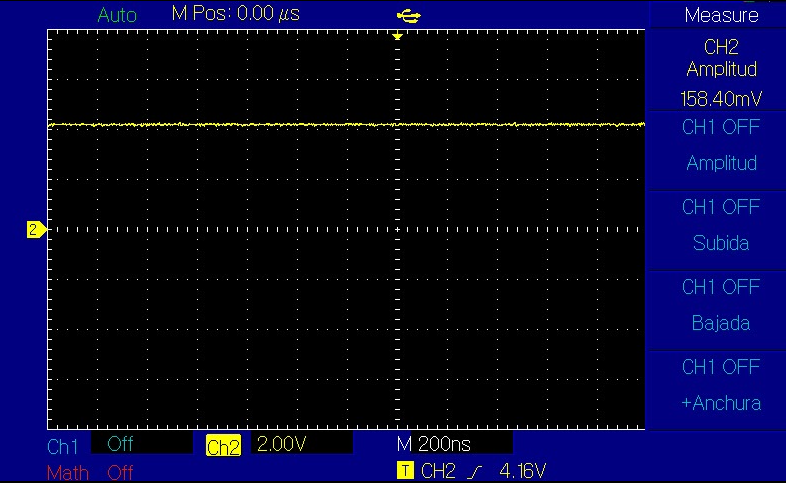
\includegraphics[width=0.7\linewidth]{imagen17.png}
            \caption{Simulación del circuito con diferentes valores de $R_2$ y su efecto en el voltaje de rizado.}
            \label{fig:simulacion_rizado_R2}
        \end{figure}

\end{enumerate}

\tituloSeccion{Conclusiones}
\begin{itemize}
    \item Se estudió el comportamiento de diodos semiconductores: se contrastó la teoría (Ecuación de Shockley) con la curva I–V medida (Análisis de datos, Paso 1, figura \ref{fig:curva_diodo}), observándose un umbral cercano a $0{,}7\,$V y la diferencia entre regiones de polarización directa e inversa. 
    \item Se analizó el diodo en circuito alimentado por fuente AC: en los Pasos 1 a 3 se registraron curvas y formas de onda (figs. \ref{fig:rectificador_medio_onda}, \ref{fig:salida_medio_onda}, \ref{fig:salida_medio_onda_fuente}), se midieron los voltajes pico (entrada $\approx5\,$V, salida $\approx4{,}3\,$V) y se verificó el efecto de recorte/clipper descrito en el procedimiento. La comparación entre configuraciones (incluida la inversión del diodo en Paso 3) permitió entender el impacto de la polaridad en la forma de salida y su potencial uso en recorte o protección de señales.
    \item Se estudiaron los rectificadores de media onda y de onda completa y el efecto del filtro capacitivo: los Pasos 4 y 5 y las figuras \ref{fig:entrada_onda_completa}, \ref{fig:salida_onda_completa}, \ref{fig:salida_onda_completa_filtro}, junto con la expresión $V_r\approx\dfrac{V_{DC}}{2fR_LC}$ y los cálculos para $C=1,\,10,\,47\,\mu$F, muestran la reducción del rizado al aumentar la capacitancia; las mediciones con distintos $R_2$ (Actividades adicionales) confirmaron la tendencia y permitieron estimar el factor de rizado. En la práctica, para las condiciones del experimento se recomienda optar por capacitancias del orden de $10\!\sim\!47\,\mu$F para obtener un rizado reducido sin sobredimensionar los componentes.
\end{itemize}

\tituloSeccion{Bibliografía}
\begin{enumerate}[label={[\arabic*]}]
	\item R. L. Boylestad, \textit{Introducción al análisis de circuitos}, 12.\textsuperscript{a} ed. México: Pearson Education/Prentice Hall, 2010.
    \item UNI-FC, \textit{Circuitos Electrónicos Analógicos: Guía de laboratorio del experimento 5}. Lima, Perú, 2026.
\end{enumerate}
\newpage

\section{Anexos}
\begin{figure}[H]
    \centering
    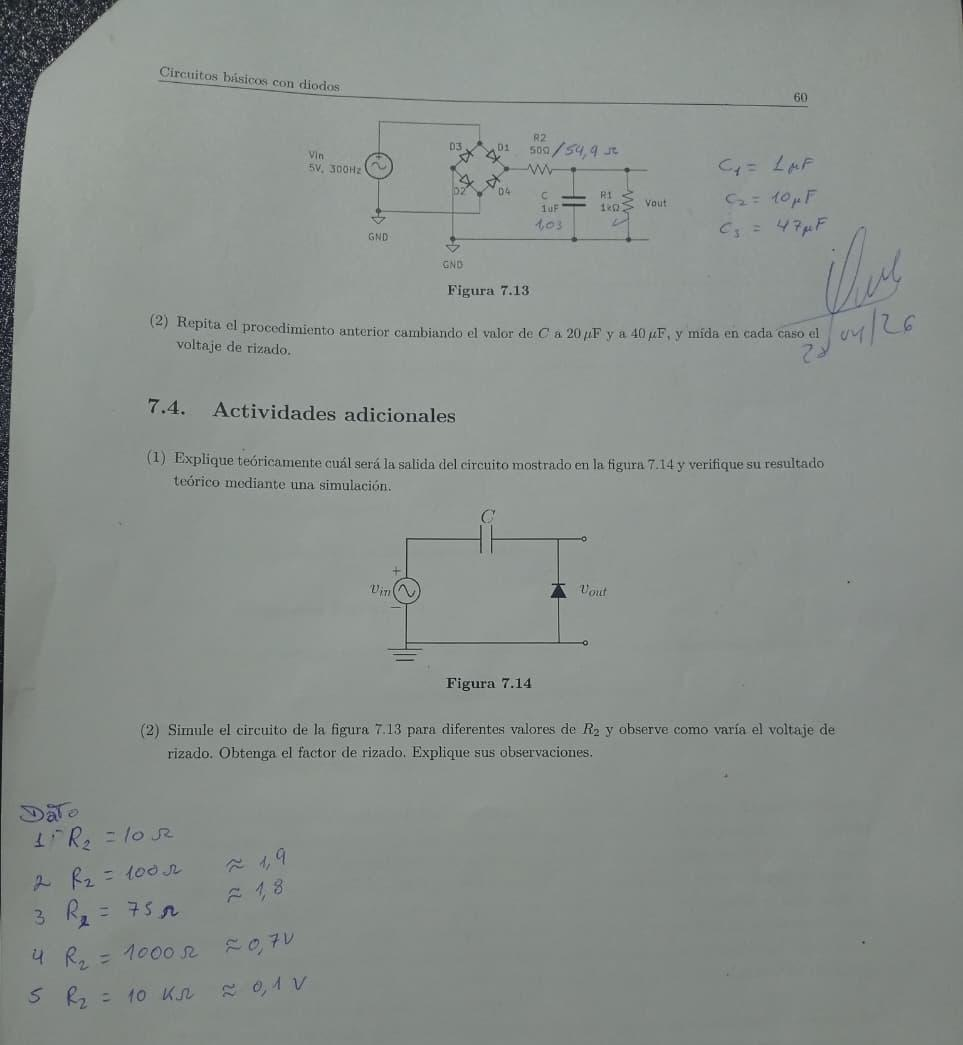
\includegraphics[width=0.55\linewidth]{imagen18.jpeg}
    \caption{Hoja de datos.}
    \label{fig:anexo_paso1}
\end{figure}
\end{document}